\documentclass[UTF8,a4paper,12pt,fontset=fandol]{ctexart}

\usepackage[left=2.5cm,right=2.5cm,top=2.6cm,bottom=2.6cm]{geometry}
\usepackage{amsmath,amssymb,amsthm,bm}
\usepackage{booktabs,multirow,array}
\usepackage{graphicx}
\graphicspath{{figures/}}
\usepackage{caption}
\usepackage{enumitem}
\usepackage{hyperref}
\usepackage[numbers,sort&compress]{natbib}

\hypersetup{
  colorlinks=true,
  linkcolor=black,
  citecolor=black,
  urlcolor=blue
}

\title{面向干扰耦合5G微基站网络的双时间尺度切片与功率协同优化方法}
\author{作者待补}
\date{\today}

\begin{document}

\maketitle

\begin{abstract}
5G网络切片需要在同一无线接入基础设施上同时承载URLLC、eMBB和mMTC三类异构业务。本文关注预设微基站仿真场景中的三个耦合难点：$1\,\mathrm{ms}$任务服务粒度与$100\,\mathrm{ms}$切片重配置周期并存、RB预算必须满足业务颗粒度约束、多微基站同频传输引入功率--干扰耦合。为此，本文构建双时间尺度切片与功率协同优化模型，并采用三层递进式求解链：静态单站枚举用于校准模型闭合性，动态单站有限时域滚动优化用于建立可解释基线，多站干扰场景下采用``切片层离散预算+功率层连续控制''的分层PPO求解器。实验表明，动态单站中$lookahead=2$在考察的$H\in\{1,2,3\}$内取得最高目标值$0.8986$；多站场景中分层PPO在三组随机种子下达到$0.4960\pm0.0031$的综合目标值，高于均匀分配基线（$0.4740$）和轻量级层次AC基线（$0.4553$）。最佳模型实现URLLC零丢弃，eMBB平均时延紧贴$100\,\mathrm{ms}$门限，mMTC完成率约50\%。功率层使平均发射功率由固定$30\,\mathrm{dBm}$设置下的约$9.0000\,\mathrm{W}$降至$0.1032\,\mathrm{W}$，但服务目标仅提升约$0.0020$，说明其当前贡献主要体现为近似不损失服务质量的低功率可行控制，而非显著QoS增益。
\end{abstract}

\noindent\textbf{关键词：}5G网络切片；双时间尺度优化；资源块分配；功率控制；分层强化学习

\section{引言}

5G网络切片在同一物理基础设施上同时承载URLLC（低时延高可靠）、eMBB（高吞吐宽带）和mMTC（海量接入）三类业务。它们的时延、速率和接入需求差异显著，使得无线资源管理不再是单一的频谱分配问题，而是一个需同时处理业务隔离、服务保障和跨站协调的多目标优化问题。

在无线接入侧，切片资源管理受到三个结构性难点的共同制约。其一，业务队列和信道状态持续演化，资源决策必须具备时间前瞻性。其二，系统重配置发生在较粗的$100\,\mathrm{ms}$粒度上，但URLLC的时延约束仅为$5\,\mathrm{ms}$，形成明显的双时间尺度耦合——若只在$100\,\mathrm{ms}$粒度上建模，URLLC约束无法表达；若按$1\,\mathrm{ms}$做全局联合优化，状态和动作空间会迅速膨胀。其三，在多微基站同频部署下，任一基站的发射功率都会通过同频干扰改变其他链路的信干噪比，即干扰耦合。这三个难点必须同时处理：如果只考虑双时间尺度而忽略干扰协调，多站场景中功率会过度注入导致SINR恶化；如果只做功率控制而不纳入切片预算，则无法回答``频谱资源如何在业务间切分''这一问题。

现有工作已从不同角度触及上述难点。Su等和S{\'a}nchez等的综述指出，切片资源管理的核心在于隔离性、可编排性和多目标约束下的资源协调，并认为深度强化学习特别适合处理动态、不完全可观测的长期资源控制问题\cite{su2019survey,sanchez2022survey}。在分层方法方面，Chen等提出了基于深度强化学习的双层切片资源分配框架\cite{chen2022two_tier}，Jiang等在MEC场景中构建了``服务层切片+动态资源分配''两级强化学习体系\cite{jiang2024rlsa}。这些工作验证了分层分解路线的合理性，但Chen等侧重切片资源竞价，Jiang等侧重MEC通信--计算资源，均未同时处理本文场景中的固定RB颗粒度、微基站干扰耦合、功率控制和三类切片任务级SLA评价。

综上，当前缺少一套面向无线接入侧、能够同时处理异构切片SLA、双时间尺度任务演化、固定RB颗粒度以及多微基站干扰与功率控制耦合的统一方法。本文要回答的核心问题是：在$100\,\mathrm{ms}$切片重配置周期、$1\,\mathrm{ms}$任务服务粒度和多基站同频干扰的约束下，切片RB预算与发射功率应如何协同决策，才能最大化三类切片的长期加权平均服务质量？

本文的贡献如下：

\begin{enumerate}[leftmargin=2em]
  \item 构建了面向5G微基站无线接入侧的双时间尺度切片资源模型，将$100\,\mathrm{ms}$切片重配置与$1\,\mathrm{ms}$任务执行统一到一个优化框架中，同时纳入RB颗粒度约束、异构SLA和跨站干扰耦合。
  \item 设计了从枚举校准、有限时域滚动优化到分层PPO的递进式求解链：静态场景验证模型闭合性，动态单站场景建立可解释的时间前瞻基线，完整多站场景采用``上层离散切片预算+下层连续功率控制''的分层PPO求解。
  \item 在预设仿真场景上验证了框架有效性：动态单站中$lookahead=2$在$H\in\{1,2,3\}$内取得最高目标值；多站中分层PPO在三组随机种子下稳定优于轻量级层次基线和均匀分配基线；参数灵敏度分析显示主要现象在已考察扰动范围内保持相对稳定。同时，消融实验表明功率层主要体现为低功率可行控制（目标值增量约$0.002$），mMTC完成率仅约50\%，为后续改进指出了明确方向。
\end{enumerate}

\begin{figure}[htbp]
  \centering
  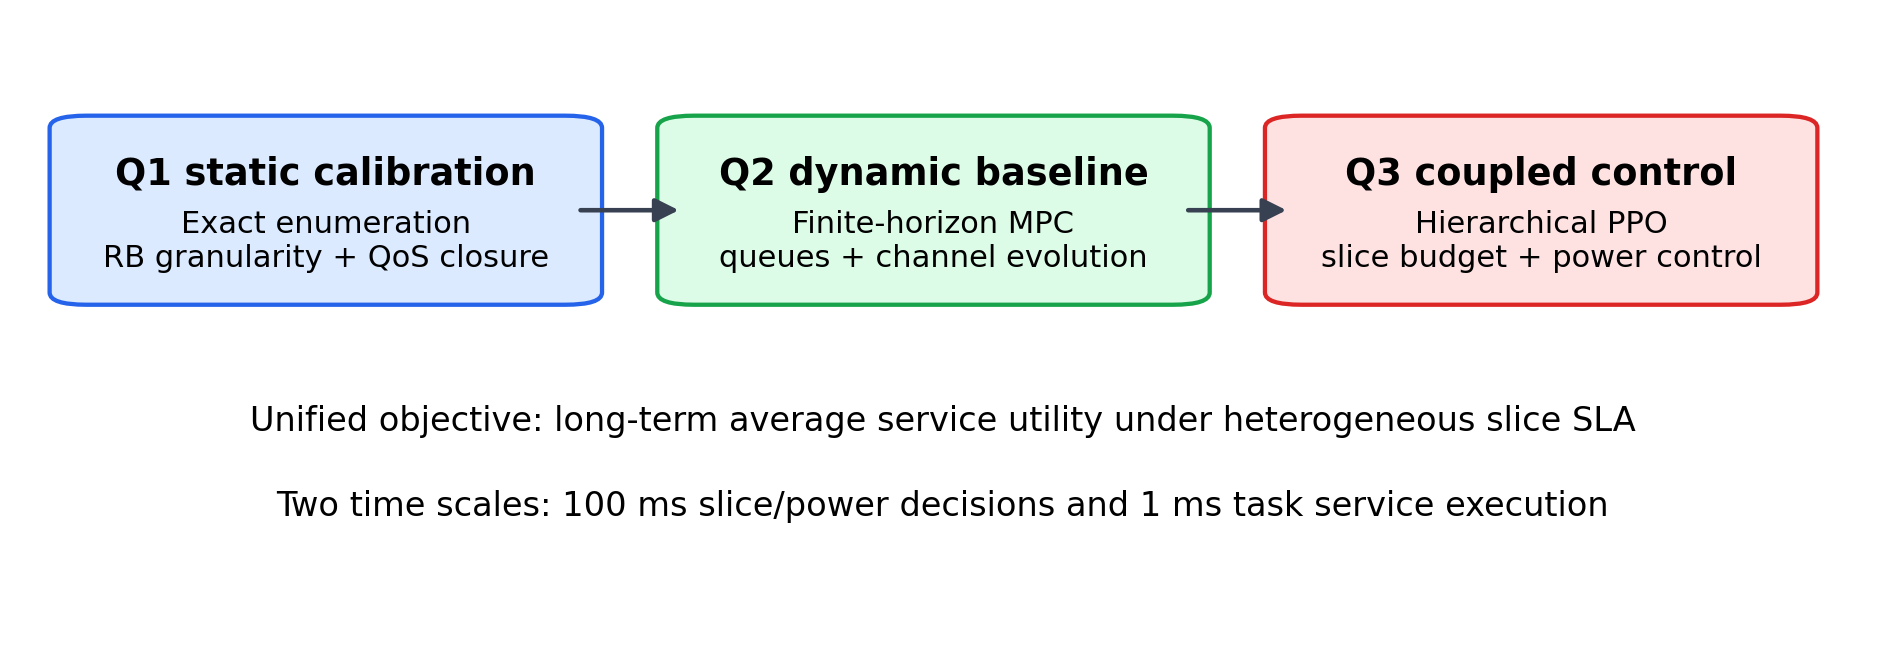
\includegraphics[width=0.98\linewidth]{framework.png}
  \caption{三层递进式证据链：静态校准（模型闭合性）、动态基线（时间前瞻价值）、多站耦合控制（完整问题求解）。}
  \label{fig:framework}
\end{figure}

\section{相关工作}

已有研究可归为三条与本文密切相关的技术路线。

\textbf{切片资源分配框架。} Su等和S{\'a}nchez等的综述指出，切片资源管理的核心不仅是频谱切分，还包括对不同业务时延、速率和可靠性偏好的统一表示，并认为DRL适合处理该类问题\cite{su2019survey,sanchez2022survey}。这类工作为本文提供了问题分类和建模背景。

\textbf{分层或双层切片控制。} Chen等在无线接入网络中提出了基于DRL和联合竞价的双层切片资源分配机制\cite{chen2022two_tier}；Jiang等在MEC场景中使用两级强化学习分别处理服务层切片和动态资源分配\cite{jiang2024rlsa}。这些工作启发了本文将问题拆解为慢时间尺度预算决策和快时间尺度功率执行两个层级，但本文没有照搬其MEC计算资源块设定，而是将下层重新映射为无线接入侧的功率控制与干扰协调。

\textbf{干扰耦合与功率变量。} 在多微基站同频部署下，路径损耗、小尺度衰落和跨站干扰共同决定链路SINR，这一物理约束与3GPP信道建模思想一致\cite{3gpp38901}。本文将功率控制纳入完整问题，是为了匹配第三层多站干扰场景的决策变量；但实验结果显示，当前功率层主要带来低功率可行性，而不是主要服务质量增益，因此相关结论在后文按受限口径报告。

表\ref{tab:related_work}给出代表性工作对比。该表用于说明本文的问题定位，不构成系统性综述，也不声称穷尽已有方法。

\begin{table}[htbp]
  \centering
  \caption{与代表性相关工作的定位对比}
  \label{tab:related_work}
  \resizebox{\linewidth}{!}{%
  \begin{tabular}{lllllll}
    \toprule
    工作 & 主要对象 & 双时间尺度 & 异构SLA & RB颗粒度 & 干扰/功率耦合 & 与本文关系 \\
    \midrule
    Su et al.\cite{su2019survey} & 切片资源综述 & -- & \checkmark & -- & -- & 问题背景 \\
    S{\'a}nchez et al.\cite{sanchez2022survey} & DRL切片综述 & -- & \checkmark & -- & -- & 方法背景 \\
    Chen et al.\cite{chen2022two_tier} & 无线接入切片 & -- & \checkmark & \checkmark & -- & 双层切片启发 \\
    Jiang et al.\cite{jiang2024rlsa} & MEC切片与资源分配 & \checkmark & \checkmark & -- & -- & 分层RL启发 \\
    本文 & 微基站无线接入 & \checkmark & \checkmark & \checkmark & \checkmark & 任务场景求解 \\
    \bottomrule
  \end{tabular}}
\end{table}

\section{系统模型与问题表述}

\noindent\textbf{符号表。} 为便于阅读，表\ref{tab:notation}集中列出本文核心符号。

\begin{table}[htbp]
  \centering
  \caption{核心符号表}
  \label{tab:notation}
  \small
  \begin{tabular}{cll}
    \toprule
    符号 & 含义 & 单位/取值范围 \\
    \midrule
    $B$ & 微基站数量 & 多站实验取 $B=3$ \\
    $R^{\max}$ & 每基站总RB数 & 50 \\
    $W_{\text{RB}}$ & 单RB带宽 & $360\,\mathrm{kHz}$ \\
    $s\in\{u,e,m\}$ & 切片类型：URLLC/eMBB/mMTC & -- \\
    $x_{b,s,t}$ & 周期$t$基站$b$给切片$s$分配的RB数 & $\{0,\dots,50\}$ \\
    $g_s$ & 切片$s$每任务RB占用量 & $u/e/m:10/5/2$ \\
    $n_{b,s,t}$ & 切片$s$可并行服务的最大用户数 & $\lfloor x_{b,s,t}/g_s\rfloor$ \\
    $P_{b,s,t}^{\text{dBm}}$ & 发射功率 & $[10,30]\,\mathrm{dBm}$ \\
    $L_{i,b,t}$ & 大尺度路径损耗 & dB \\
    $h_{i,b,t}$ & 小尺度瑞利衰落 & 复数 \\
    $N_{0,s}^{\mathrm{mW}}$ & 切片$s$占用带宽下的噪声功率 & mW \\
    $\mathrm{SINR}_{i,b,t}$ & 用户$i$在基站$b$处的信干噪比 & 线性 \\
    $r_{i,b,t}$ & 用户$i$瞬时速率 & bps \\
    $\tau_s^{\max}$ & 切片$s$的时延上限 & $\{5,100,500\}\,\mathrm{ms}$ \\
    $C_s^{\min}$ & 切片$s$的速率目标 & $\{10,50,1\}\,\mathrm{Mbps}$ \\
    $\alpha_u$ & URLLC时延折扣因子 & 0.95 \\
    $\beta_s$ & 切片$s$的超时惩罚系数 & $\{5,3,1\}$ \\
    $w_s$ & 切片$s$的权重 & $1/3$ \\
    $J$ & 系统目标值（加权切片效用） & -- \\
    \bottomrule
  \end{tabular}
\end{table}

\subsection{网络场景与数据来源}

本文研究对象为由$B$个微基站构成的5G无线接入网络，在完整多站实验中取$B=3$。每个微基站持有50个资源块；单个资源块的频域带宽为$360\,\mathrm{kHz}$，服务粒度为$1\,\mathrm{ms}$，二者为本文预设仿真场景中的资源粒度设定，并与5G NR物理资源块化建模思想一致\cite{3gpp38211}。信道模型考虑大尺度路径损耗与小尺度瑞利衰落，其物理语义参考3GPP TR 38.901\cite{3gpp38901}。用户位置、信道数据与任务到达流采用预设仿真场景数据；因此本文定位为基于仿真的方法研究，而非现场测量研究。

\subsection{双时间尺度建模}

预设场景中系统每$100\,\mathrm{ms}$决策一次资源配置方案，而任务的排队、占用与释放以$1\,\mathrm{ms}$为基本执行粒度。因此本文将系统控制划分为两个时间层次：

\begin{itemize}[leftmargin=2em]
  \item 慢时间尺度：每$100\,\mathrm{ms}$做一次切片资源预算更新；在多基站场景下同时更新基站--切片发射功率；
  \item 快时间尺度：在每个$1\,\mathrm{ms}$微时隙内，根据当前切片预算与信道状态推进任务服务、队列变化和资源释放。
\end{itemize}

这一建模方式的必要性在于：若只保留$100\,\mathrm{ms}$粒度，则URLLC的$5\,\mathrm{ms}$时延约束无法被正确表达；若完全按$1\,\mathrm{ms}$做全局联合优化，则状态与动作空间会迅速膨胀，导致求解代价难以接受。

\subsection{切片业务与参数标定}

本文考虑三类切片业务：URLLC、eMBB和mMTC。其业务语义锚定于3GPP中对低时延高可靠、高吞吐宽带和大连接低速率业务的定义\cite{3gpp23501,3gpp22261}，但实验中的具体数值采用本文仿真场景设定，而不将其表述为某一单一标准5QI条目的直接拷贝。三类业务的参数见表\ref{tab:slice_params}。

\begin{table}[htbp]
  \centering
  \caption{三类切片的业务语义与场景参数化}
  \label{tab:slice_params}
  \resizebox{\linewidth}{!}{%
  \begin{tabular}{cccccc}
    \toprule
    切片 & RB占用量 & 速率目标(Mbps) & 时延上限(ms) & 惩罚系数$\beta_s$ & 其他说明 \\
    \midrule
    URLLC & 10 & 10 & 5 & 5 & 时延折扣$\alpha_u=0.95$ \\
    eMBB & 5 & 50 & 100 & 3 & 吞吐优先 \\
    mMTC & 2 & 1 & 500 & 1 & 接入优先 \\
    \bottomrule
  \end{tabular}}
\end{table}

其中，RB占用量、时延上限与速率目标为本文仿真场景设定，$\alpha_u=0.95$与$\beta=(5,3,1)$为实验评价函数中的校准常数。需要说明的是，这些常数并非3GPP标准中特定5QI条目的直接引用，而是用于刻画三类业务差异化违约代价强度的一组场景化参数。后文参数灵敏度分析将验证主要结论对这组常数的稳健性。

\subsection{切片资源预算约束}

设第$t$个慢时间尺度决策周期内，基站$b$分配给切片$s\in\{u,e,m\}$的资源块数量为$x_{b,s,t}$，则有
\begin{equation}
  \sum_{s\in\{u,e,m\}} x_{b,s,t} \le R^{\max}=50,\quad \forall b,t.
\end{equation}
同时，切片资源预算必须满足颗粒度约束
\begin{equation}
  x_{b,u,t}\in 10\mathbb{Z}_+,\qquad
  x_{b,e,t}\in 5\mathbb{Z}_+,\qquad
  x_{b,m,t}\in 2\mathbb{Z}_+.
\end{equation}
因此，每个切片在单个微时隙内可并行服务的最大用户数为
\begin{equation}
  n_{b,s,t} = \left\lfloor \frac{x_{b,s,t}}{g_s}\right\rfloor,
\end{equation}
其中$g_s$表示切片$s$的每任务资源块占用量。

\subsection{传输、队列与干扰模型}

根据本文采用的信号传输模型，用户$i$在基站$b$服务下的接收信号功率为
\begin{equation}
  P^{\text{rx}}_{i,b,s,t} = 10^{\frac{P_{b,s,t}^{\text{dBm}}-L_{i,b,t}}{10}}\cdot |h_{i,b,t}|^2,
\end{equation}
其中$P_{b,s,t}^{\text{dBm}}$为dBm形式的发射功率，$L_{i,b,t}$为大尺度路径损耗，$h_{i,b,t}$为小尺度瑞利衰落。由于$0\,\mathrm{dBm}=1\,\mathrm{mW}$，上式得到的$P^{\text{rx}}$单位为mW。切片$s$占用$g_s$个RB时，噪声功率的dBm形式为
\begin{equation}
  N_{0,s}^{\text{dBm}}=-174+10\log_{10}\left(g_s W_{\text{RB}}\right)+NF,
\end{equation}
对应的mW形式为
\begin{equation}
  N_{0,s}^{\text{mW}}=10^{N_{0,s}^{\text{dBm}}/10}.
\end{equation}

若多微基站在同频资源上同时传输，干扰项同样按mW累加。设$\rho_{b,b',s,s',t}$为基站$b$的切片$s$与基站$b'$的切片$s'$在RB区间上的重叠比例，则用户$i$受到的跨站干扰为
\begin{equation}
  I_{i,b,s,t}^{\text{mW}} =
  \sum_{b'\neq b}\sum_{s'\in\{u,e,m\}}
  \rho_{b,b',s,s',t} P^{\text{rx}}_{i,b',s',t}.
\end{equation}
因此用户$i$的信干噪比为
\begin{equation}
  \mathrm{SINR}_{i,b,t} =
  \frac{P^{\text{rx}}_{i,b,s,t}}
  {I_{i,b,s,t}^{\text{mW}} + N_{0,s}^{\text{mW}}},
\end{equation}
由香农公式得到瞬时速率
\begin{equation}
  r_{i,b,t}=g_s W_{\text{RB}}\log_2\bigl(1+\mathrm{SINR}_{i,b,t}\bigr).
\end{equation}

第1、2层场景采用固定发射功率$30\,\mathrm{dBm}$；第3层场景中允许每个基站每类切片的发射功率在$10$至$30\,\mathrm{dBm}$之间调节，即
\begin{equation}
  P_{b,s,t}^{\text{dBm}}\in [10,30].
\end{equation}

在任务流程上，切片预算先于微时隙执行确定；任务到达后进入所属切片队列，按编号顺序和RB可用性依次占用资源块并接受服务，完成后释放资源。对于动态场景，队列状态在每个微时隙内更新；对于多基站场景，当前实现采用最近微基站接入作为显式建模假设，接入模式优化不纳入本文研究范围。

\subsection{统一效用函数}

三类切片的服务质量函数采用任务级定义。

对URLLC任务$i$，若其总时延$d_i$不超过时延上限$\tau_u^{\max}$，则其服务质量定义为
\begin{equation}
  q_i^{(u)} =
  \alpha_u^{d_i},\qquad d_i\le \tau_u^{\max};
\end{equation}
否则
\begin{equation}
  q_i^{(u)} = -\beta_u.
\end{equation}

对eMBB任务$i$，若总时延满足约束，则其服务质量按有效服务速率相对于目标速率的达成比例计算：
\begin{equation}
  q_i^{(e)}=
  \min\left(\frac{r_i^{\text{eff}}}{C_e^{\min}},1\right),\qquad d_i\le \tau_e^{\max},
\end{equation}
否则
\begin{equation}
  q_i^{(e)}=-\beta_e.
\end{equation}

对mMTC任务，大连接业务语义强调其核心是接入成功性。由于当前数据与代码采用任务级推进，因此本文将其操作化为：若任务在时延门限内完成，则计为一次成功接入并赋值1，否则记为超时惩罚
\begin{equation}
  q_i^{(m)}=
  \begin{cases}
    1, & d_i\le \tau_m^{\max},\\
    -\beta_m, & d_i> \tau_m^{\max}.
  \end{cases}
\end{equation}
该定义与附录中的``决策周期内接入比例''口径并不矛盾。若第$t$个周期内mMTC到达数为$A_{m,t}$、成功接入数为$S_{m,t}$，则成功项在全时域到达数下的归一化结果为
\begin{equation}
  \frac{1}{A_m^{\text{total}}}\sum_t S_{m,t}
  =
  \sum_{t:A_{m,t}>0} \frac{A_{m,t}}{A_m^{\text{total}}}\cdot
  \frac{S_{m,t}}{A_{m,t}},
\end{equation}
即按周期到达量加权的接入比例。失败任务的$-\beta_m$项则对应附录给定的超时惩罚，在同一任务级归一化口径下计入系统目标。

设第$t$个决策周期内切片$s$完成评估的任务集合为$\mathcal{D}_{s,t}$，对应切片权重为$w_s$。设切片$s$在整个评估时域内的任务到达总数为$A_s^{\text{total}}$，则系统目标定义为按到达总数归一化的加权切片效用：
\begin{equation}
  J = \sum_{s\in\{u,e,m\}}
  w_s\cdot \frac{1}{A_s^{\text{total}}}
  \sum_{t=1}^{T}\sum_{i\in\mathcal{D}_{s,t}} q_i^{(s)}.
  \label{eq:objective}
\end{equation}
其中$A_s^{\text{total}}$为固定常数（由数据给定），任务一旦被解析（完成或超时丢弃）即计入对应$\mathcal{D}_{s,t}$。该形式等价于按每类切片的全时域到达规模对任务级效用做加权平均，避免了因各周期解析量差异导致的估计偏差。在固定时域$T=1000\,\mathrm{ms}$的评测场景下，上式即为本文代码中实际计算的目标值。

本文默认采用等权设置$w_u=w_e=w_m=\frac{1}{3}$，并在后续通过参数灵敏度分析考察结论对校准常数扰动的稳定性。

\subsection{统一优化问题表述}

将上述约束和目标集成，本文研究的优化问题可表述为：

\begin{subequations}
\begin{align}
  \max_{\{x_{b,s,t}\},\{P_{b,s,t}\}} \quad
  & J = \sum_{s\in\{u,e,m\}} w_s\cdot \frac{1}{A_s^{\text{total}}}
        \sum_{t=1}^{T}\sum_{i\in\mathcal{D}_{s,t}} q_i^{(s)}
        \label{eq:opt_obj} \\[4pt]
  \text{s.t.} \quad
  & \sum_{s} x_{b,s,t} \le R^{\max},\quad \forall b,t \label{eq:opt_rb} \\
  & x_{b,u,t}\in 10\mathbb{Z}_+,\; x_{b,e,t}\in 5\mathbb{Z}_+,\; x_{b,m,t}\in 2\mathbb{Z}_+ \label{eq:opt_gran} \\
  & P_{b,s,t}^{\text{dBm}}\in [10,30],\quad \forall b,s,t \label{eq:opt_pow} \\
  & \text{满足上述任务服务、队列演化与干扰计算规则}.
        \label{eq:opt_env}
\end{align}
\end{subequations}

该问题的核心难点在于：决策变量同时包含离散量（$x_{b,s,t}$）和连续量（$P_{b,s,t}$）；约束中包含了由前述模型定义的、含随机队列演化和跨站干扰反馈的复杂环境动力学；且$T=1000\,\mathrm{ms}$的有限时域要求决策具备时间前瞻性。直接对该问题进行联合优化在计算上不可行，因此本文采用下一节所述的分层求解策略。

\section{求解框架}

\subsection{总体思路}

若直接在完整多站场景上对所有决策变量做一次性联合优化，问题将同时面临离散切片预算、连续功率控制、随机队列演化和跨站干扰反馈，求解代价难以接受。因此本文采用``由简入繁''的三级求解链：
\begin{enumerate}[leftmargin=2em]
  \item 在静态单站场景下，穷举切片预算并配合固定贪心调度，验证效用函数和资源约束的逻辑闭合性；
  \item 在动态单站场景下，采用有限时域滚动优化——对外层切片预算序列进行枚举搜索，内层以固定FCFS排队规则模拟$1\,\mathrm{ms}$任务服务——建立可解释的时间演化基线；
  \item 在完整多站干扰场景下，构建分层PPO求解器处理离散--连续混合动作空间。
\end{enumerate}

\subsection{静态校准层：预算枚举}

在单站单时刻场景中，三类切片在50个RB内进行整数划分，同时满足$10/5/2$的颗粒度约束。该层穷举所有21种可行的$(x_u,x_e,x_m)$组合，对每种组合采用贪心最短处理时间优先（SPT）的机器调度启发式安排任务执行顺序，计算对应的切片效用均值，选出综合目标最大的预算方案。

该层的作用不是展示算法性能，而是验证三点：(i) QoS评价函数是否与任务流程和资源颗粒度一致；(ii) 资源块粒度、速率公式和时延约束是否存在逻辑冲突；(iii) 在最简设置下，效用函数能否区分不同资源分配方案的质量差异。实现脚本为\texttt{channel\_data等2个文件/solve\_q1.py}。

\subsection{单站动态层：有限时域滚动优化}

在引入$1000\,\mathrm{ms}$时域和动态任务流后，单站场景具有明显的时序决策特征。本文在每个$100\,\mathrm{ms}$决策点采用有限时域滚动优化：枚举当前所有合法切片预算动作，对每个动作向前仿真$H$个窗口，在窗口内部以固定FCFS排队策略按$1\,\mathrm{ms}$粒度推进任务服务，选择$H$步窗口内投影累计目标值最大的动作。设当前状态为$S_t$，合法预算动作为$\mathcal{A}$，则第$t$个窗口的决策为

\begin{equation}
  a_t^\star = \arg\max_{a_t\in\mathcal{A}} \Bigl\{
    \Delta J(S_t,a_t) + \sum_{k=t+1}^{t+H-1} \Delta J\bigl(S_k,\,a_k^\star(S_k)\bigr)
  \Bigr\},
\end{equation}
其中$S_{k}$由固定FCFS服务模拟的确定性环境转移产生，$a_k^\star(S_k)$为从$S_k$出发在剩余$H-k+t-1$步内的最优预算序列（同样通过枚举获得）。对$1000\,\mathrm{ms}$终点仍未完成的任务施加终端丢弃惩罚。

该层的意义在于：它提供了一个不依赖神经网络训练、具备完全可解释性的动态单站基线，说明即使在不考虑跨站干扰时，时间前瞻本身也足以改变资源配置效果。实现脚本为\texttt{q2\_mpc.py}。

\subsection{多站耦合层：分层强化学习}

当系统扩展到多微基站同频部署时，切片预算与功率控制通过SINR中的干扰项发生耦合。若采用单层统一动作表示，将同时面临高维离散--连续混合动作空间和稀疏长期回报问题。本文借鉴Jiang等\cite{jiang2024rlsa}的两级分解思想，将其从MEC场景重新映射到无线接入侧：上层负责基站--切片的离散RB预算决策，下层负责基站--切片的连续功率控制。这一分解的合理性基于以下观察：(i) 预算决策在$100\,\mathrm{ms}$周期进行，功率控制虽然也同步更新，但干扰影响的物理时间尺度更短，将功率放在下层响应更灵活；(ii) 离散预算和连续功率在动作表征上不兼容（gym空间不支持混合类型），分层避免了手工离散化功率带来的信息损失。

\subsubsection{环境与状态空间}

多站环境的实现脚本为\texttt{q3\_hierarchical\_rl.py}（环境核心）和\texttt{q3\_sb3.py}（PPO训练入口）。环境按双时间尺度组织：每$100\,\mathrm{ms}$触发一次切片预算决策和功率控制决策，决策后窗口内的$1\,\mathrm{ms}$任务服务由环境自动推进。

上层切片策略环境$\mathcal{E}_{\text{slice}}$的观测向量为每个基站的32维特征拼接（$B=3$时共96维），包含：每个切片的队列长度、队首等待时间、平均剩余比特数、近期到达数量，以及关联用户的信道增益均值/最小值、上一步动作和功率。动作空间为21个离散预算索引（对应21种合法$(x_u,x_e,x_m)$组合）。

下层功率控制环境$\mathcal{E}_{\text{power}}$的观测在$\mathcal{E}_{\text{slice}}$基础上追加由上层给出的切片预算向量。动作为每基站每切片1维连续变量，经线性映射至$[10,30]\,\mathrm{dBm}$。

\subsubsection{评价目标与训练代理奖励}

需要区分评估口径和训练信号：式\eqref{eq:objective}中的$J$是本文所有结果表报告的官方服务目标，只由任务级服务质量、到达总数归一化和切片权重构成。PPO训练中使用代理奖励（proxy reward）以避免SLA硬约束带来的稀疏梯度问题：URLLC的任务级效用通过sigmoid函数平滑化，使其在时延接近门限时提供连续梯度信号；eMBB和mMTC同样进行平滑处理。功率正则项$-\lambda_p\sum P_{b,s,t}$、干扰正则项$-\lambda_I\sum \text{干扰比}$和公平性项只用于训练过程中的代理奖励，不混入最终报告的官方目标$J$。

\subsubsection{训练算法}

上下两层均采用近端策略优化（PPO）\cite{schulman2017ppo}。PPO的目标函数为

\begin{equation}
  \mathcal{L}^{\text{CLIP}}(\theta) =
  \hat{\mathbb{E}}_t\Bigl[
    \min\bigl(
      r_t(\theta)\hat{A}_t,\;
      \operatorname{clip}(r_t(\theta), 1-\epsilon, 1+\epsilon)\hat{A}_t
    \bigr)
  \Bigr],
\end{equation}
其中$r_t(\theta)=\pi_\theta(a_t|s_t)/\pi_{\theta_{\text{old}}}(a_t|s_t)$为策略概率比，$\hat{A}_t$为广义优势估计（GAE），$\epsilon=0.2$为裁剪参数。价值函数通过均方误差拟合：

\begin{equation}
  \mathcal{L}^{\text{VF}}(\phi) = \hat{\mathbb{E}}_t\bigl[(V_\phi(s_t) - \hat{R}_t)^2\bigr].
\end{equation}

总损失为$\mathcal{L} = \mathcal{L}^{\text{CLIP}} - c_1 \mathcal{L}^{\text{VF}} + c_2 S[\pi_\theta]$，其中$S[\pi_\theta]$为策略熵正则项。

训练采用分层序贯方式：先固定功率为$30\,\mathrm{dBm}$训练切片层PPO（\texttt{q3\_sb3.py train-slice}），再以训练好的切片模型为条件训练功率层PPO（\texttt{q3\_sb3.py train-power}），最后将两层组合进行评估。训练超参数见表\ref{tab:ppo_params}。

\begin{table}[htbp]
  \centering
  \caption{PPO训练超参数}
  \label{tab:ppo_params}
  \begin{tabular}{cc}
    \toprule
    参数 & 取值 \\
    \midrule
    学习率 & $3\times10^{-4}$ \\
    $\text{n\_steps}$（每轮收集步数）& 128 \\
    $\text{batch\_size}$ & 64 \\
    折扣因子 $\gamma$ & 0.98 \\
    GAE $\lambda$ & 0.95 \\
    裁剪范围 $\epsilon$ & 0.2 \\
    $\text{ent\_coef}$ & 0.01 \\
    $\text{vf\_coef}$ & 0.5 \\
    网络结构 & [256, 256] \\
    训练步数（切片层/功率层）& 10000 \\
    \bottomrule
  \end{tabular}
\end{table}

\section{实验设置与结果分析}

\subsection{实验数据与评价口径}

实验数据均来自项目仓库中的预设仿真场景文件。需要说明的是：静态单站（Q1）使用\texttt{channel\_data等2个文件/channel\_data.xlsx}（单时隙快照），动态单站（Q2）使用\texttt{channel\_data等2个文件(1)/channel\_data.xlsx}（$1000\,\mathrm{ms}$时域数据），多站（Q3）使用\texttt{BS2等5个文件/BS1.xlsx}、\texttt{BS2等5个文件/BS2.xlsx}、\texttt{BS2等5个文件/BS3.xlsx}和\texttt{BS2等5个文件/taskflow.xlsx}。Q1和Q2使用不同数据源，是因为Q1的作用仅是验证效用函数和资源约束的逻辑自洽性（与具体数据无关的模型校验），而Q2需要在动态时域上建立基线。三个场景共同验证同一个研究命题——双时间尺度切片预算与功率控制如何提升长期服务质量——但其数据路径独立。

评价指标包括：综合目标值$J$，各切片完成任务数和丢弃任务数，各切片平均时延，eMBB平均服务速率，以及多站场景下的平均发射功率和平均干扰比。全文中所有目标值统一保留4位小数，时延保留2位，百分比保留1位。

\subsection{静态单站校准实验}

在静态单站场景中，对21种可行$(x_u,x_e,x_m)$组合进行穷举（配合固定SPT贪心调度），结果见表\ref{tab:q1_static}。在默认等权设置下存在三组并列最优分配，综合目标值均为$0.9808$。

\begin{table}[htbp]
  \centering
  \caption{静态单站最优分配（并列三组）}
  \label{tab:q1_static}
  \begin{tabular}{cccccc}
    \toprule
    $(x_u,x_e,x_m)$ & $Q_u$ & $Q_e$ & $Q_m$ & $J$ \\
    \midrule
    (30,10,10) & 0.9935 & 0.9488 & 1.0000 & 0.9808 \\
    (20,20,10) & 0.9935 & 0.9488 & 1.0000 & 0.9808 \\
    (20,10,20) & 0.9935 & 0.9488 & 1.0000 & 0.9808 \\
    \bottomrule
  \end{tabular}
\end{table}

三组等效最优解说明当前静态场景资源尚未紧张到使最优解唯一，模型适合作为效用校准和可行性验证，但不适合作为全文的性能展示。这一现象也验证了递进式设计的必要性：若只停留在静态校准，无法体现动态队列和干扰耦合对资源管理的影响。

\begin{figure}[htbp]
  \centering
  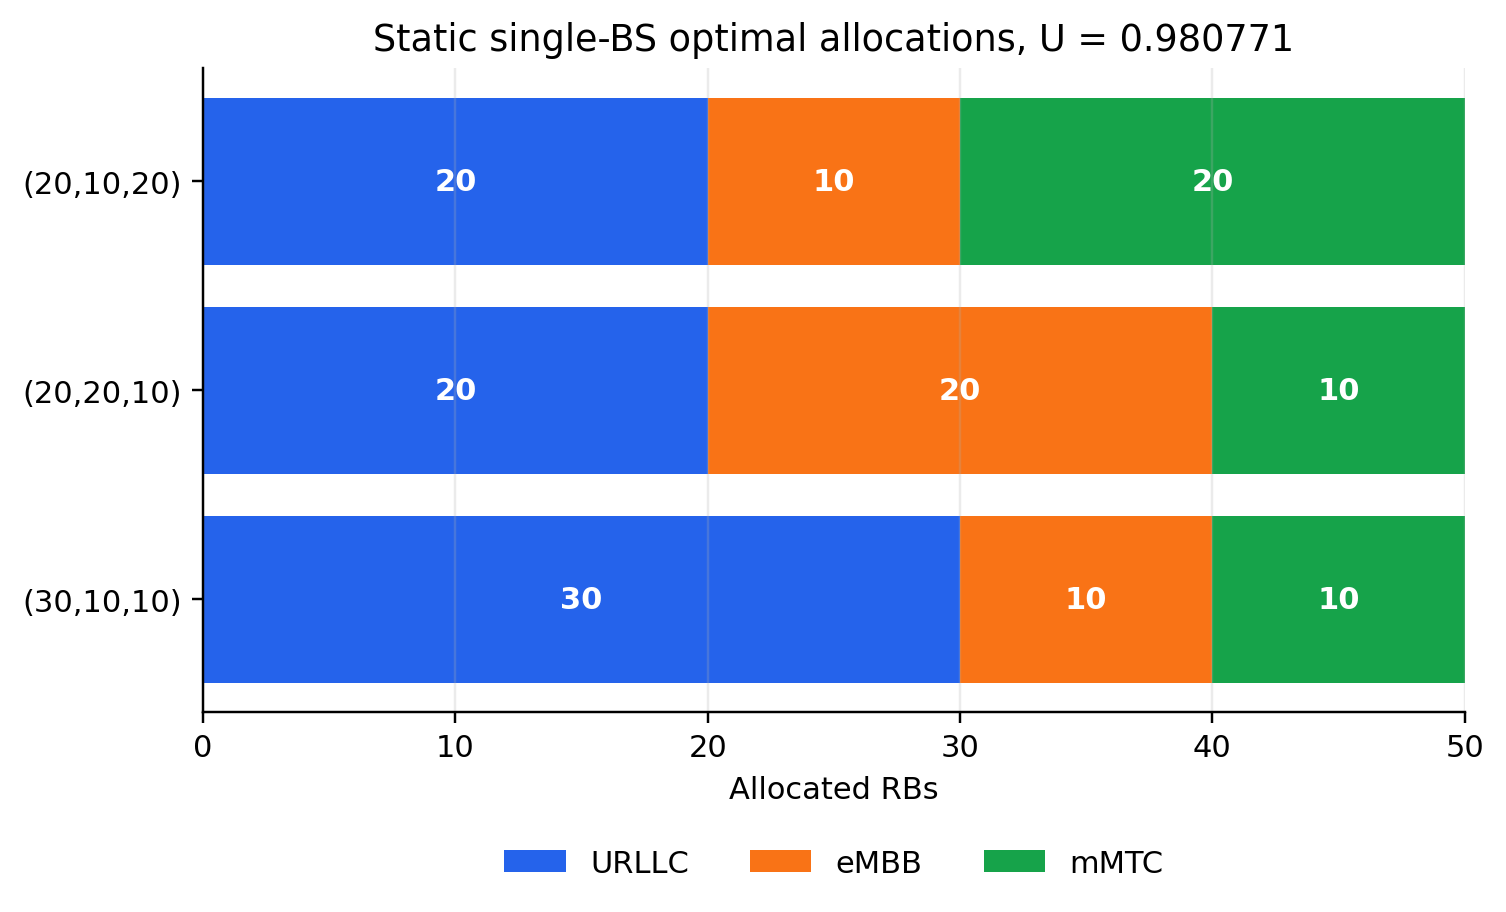
\includegraphics[width=0.72\linewidth]{q1_static_optima.png}
  \caption{静态单站场景中三组并列最优RB划分。}
  \label{fig:q1_static_optima}
\end{figure}

\subsection{动态单站对照实验}

动态单站场景通过\texttt{q2\_mpc.py}实现有限时域滚动优化，在不同前瞻深度下的结果见表\ref{tab:q2_lookahead}。

\begin{table}[htbp]
  \centering
  \caption{不同前瞻深度下的动态单站结果}
  \label{tab:q2_lookahead}
  \begin{tabular}{ccccc}
    \toprule
    前瞻深度 & 目标值 & 运行时间(s) & URLLC丢弃 & eMBB丢弃 \\
    \midrule
    $1$ & 0.8493 & $\sim$5 & 1 & 47 \\
    $2$ & 0.8986 & 36.1 & 1 & 25 \\
    $3$ & 0.8877 & 645.6 & 1 & 33 \\
    \bottomrule
  \end{tabular}
\end{table}

从$lookahead=1$到$lookahead=2$，目标值从$0.8493$升至$0.8986$，eMBB丢弃数从47降至25，说明适度前瞻改善了资源配置效果。但$lookahead=3$时目标值降至$0.8877$且运行时间增加17倍，呈明显的边际收益递减。更深层的预测在当前数据下未能带来额外收益，但搜索代价急剧放大。

\begin{figure}[htbp]
  \centering
  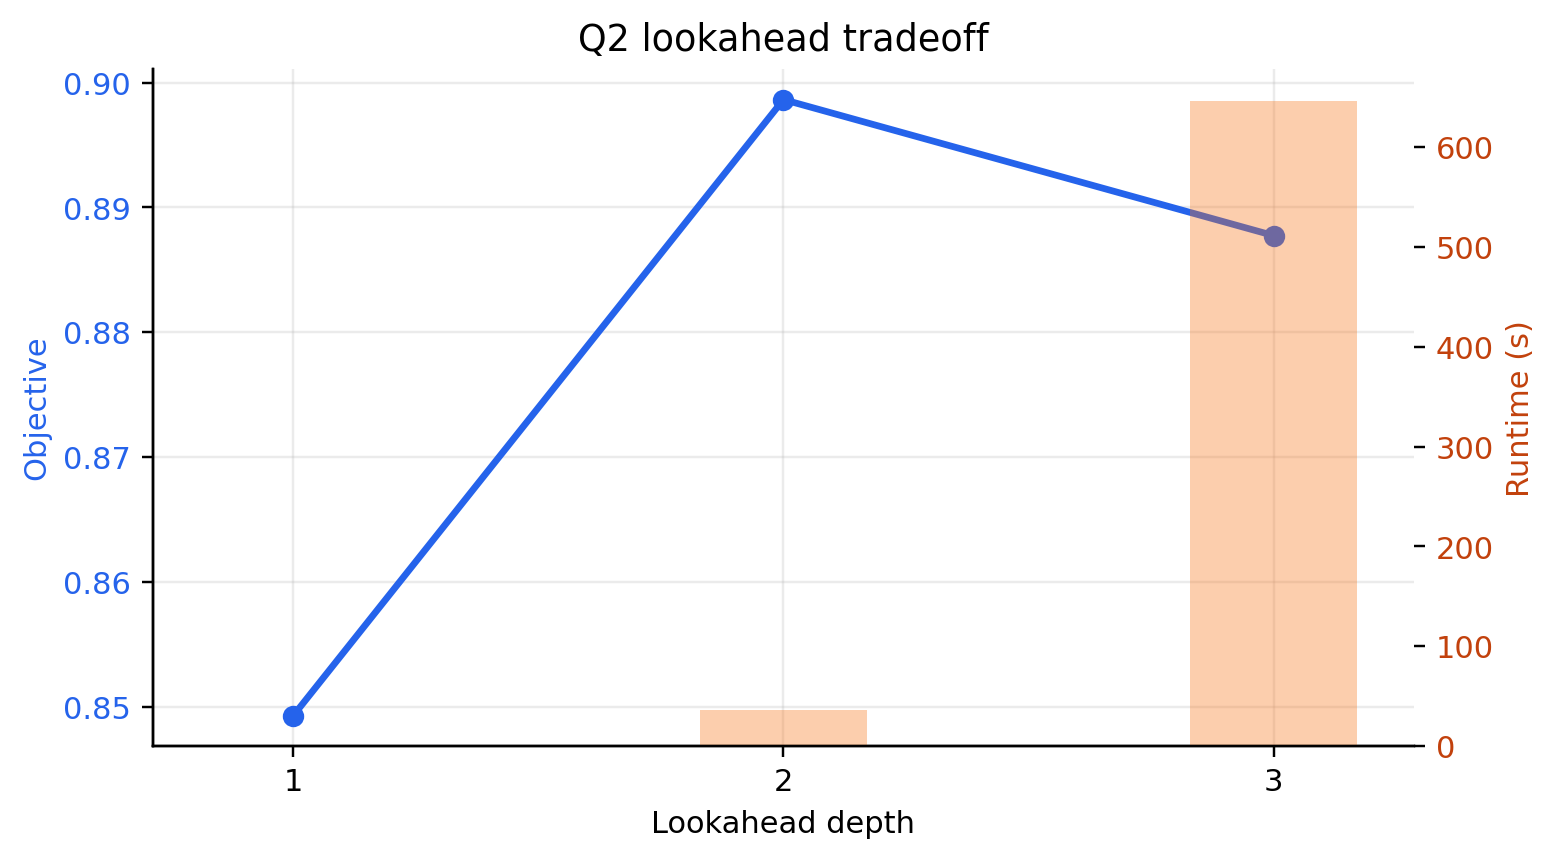
\includegraphics[width=0.72\linewidth]{q2_lookahead_tradeoff.png}
  \caption{前瞻深度对目标值与运行时间的影响：$lookahead=2$在$H\in\{1,2,3\}$中取得较好折中。}
  \label{fig:q2_lookahead_tradeoff}
\end{figure}

以$lookahead=2$为例，各切片表现为：URLLC完成216、丢弃1、平均时延$2.50\,\mathrm{ms}$；eMBB完成1931、丢弃25、平均时延$16.72\,\mathrm{ms}$；mMTC完成7010、丢弃0、平均时延$15.80\,\mathrm{ms}$。滚动优化在无干扰的单站条件下已能有效平衡三类切片的竞争，为多站强化学习层提供了可解释的强基线。

\begin{figure}[htbp]
  \centering
  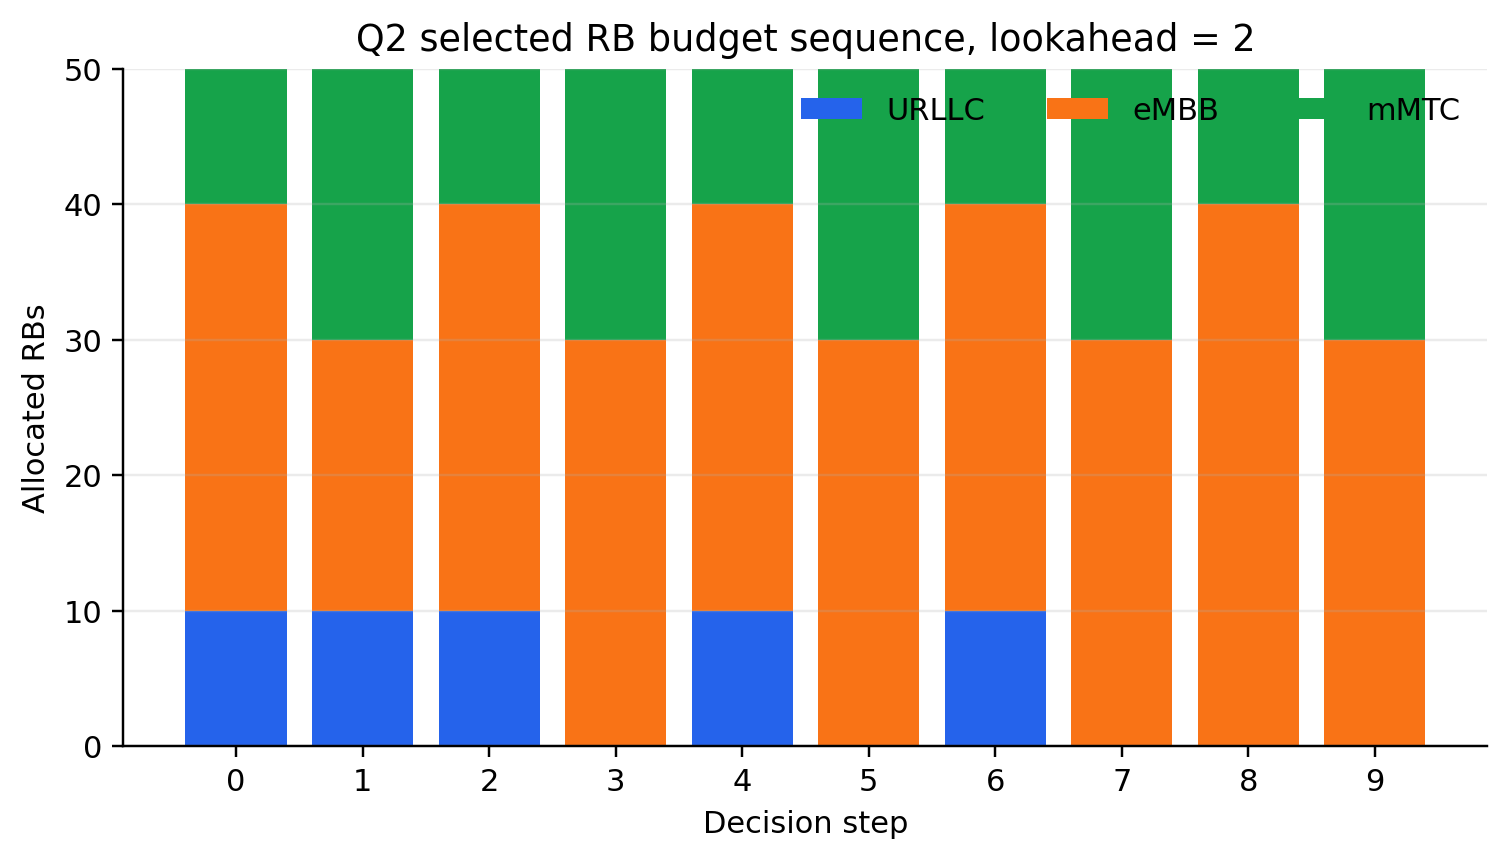
\includegraphics[width=0.76\linewidth]{q2_decision_sequence.png}
  \caption{$lookahead=2$时10个决策窗口内的RB预算序列。滚动优化随队列压力在eMBB和mMTC之间动态重分配资源。}
  \label{fig:q2_decision_sequence}
\end{figure}

\subsection{多站干扰耦合实验}

多站场景由\texttt{q3\_hierarchical\_rl.py}（环境核心）与\texttt{q3\_sb3.py}（PPO训练入口）完成训练和评估。表\ref{tab:q3_multi_seed}给出了多随机种子评估结果，同时列出两个非学习基线。

\begin{table}[htbp]
  \centering
  \caption{多站场景主结果与基线对比}
  \label{tab:q3_multi_seed}
  \begin{tabular}{ccc}
    \toprule
    方法 & 目标值 & 说明 \\
    \midrule
    均匀分配+固定功率 & 0.4740 & 非学习基线1 \\
    轻量级层次AC (numpy) & 0.4553 & 非学习基线2 \\
    \textbf{分层PPO, seed=7} & \textbf{0.4919} & -- \\
    \textbf{分层PPO, seed=17} & \textbf{0.4995} & 最佳模型 \\
    \textbf{分层PPO, seed=27} & \textbf{0.4965} & -- \\
    \midrule
    PPO 均值$\pm$标准差 & $0.4960\pm0.0031$ & 三组种子 \\
    \bottomrule
  \end{tabular}
\end{table}

三点观察：(1) 分层PPO在三组随机种子下均优于两个非学习基线，均值$0.4960$较均匀分配的$0.4740$和线性AC的$0.4553$有稳定提升；(2) 三种子间标准差为$0.0031$，说明结果不完全依赖单次初始化；(3) 均匀分配（$0.4740$）优于线性AC（$0.4553$），说明该轻量级线性逼近基线在当前环境中未能学到有效改进。

以最佳模型（seed=17）为例：综合目标值$0.4995$；URLLC完成559、丢弃0、平均时延$1.28\,\mathrm{ms}$；eMBB完成5406、丢弃587、平均时延$99.94\,\mathrm{ms}$；mMTC完成10527、丢弃10556、平均时延$398.58\,\mathrm{ms}$；eMBB平均服务速率$112.23\,\mathrm{Mbps}$；平均发射功率$0.1032\,\mathrm{W}$；平均干扰比$0.3555$。

\begin{figure}[htbp]
  \centering
  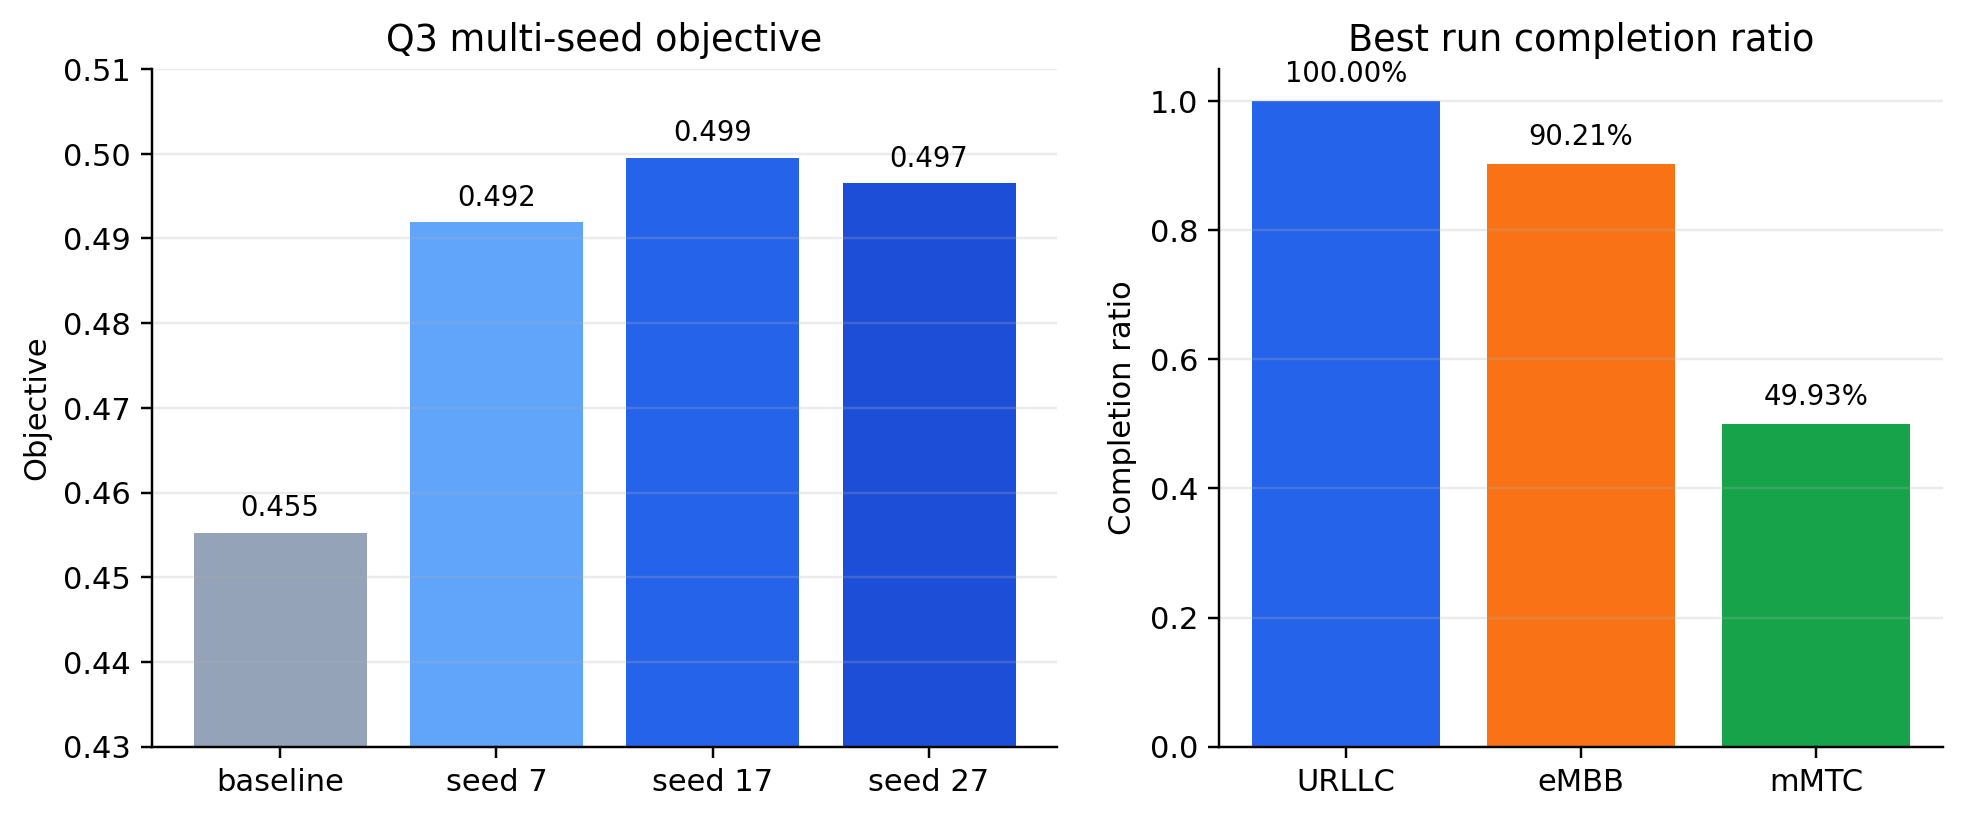
\includegraphics[width=0.90\linewidth]{q3_multiseed_summary.png}
  \caption{多站场景中多方法目标值对比与最佳模型完成率。基线为均匀分配和轻量级层次AC。}
  \label{fig:q3_multiseed_summary}
\end{figure}

\subsection{消融实验}

表\ref{tab:q3_ablation}给出功率层消融。切片层单独评估（固定$30\,\mathrm{dBm}$，不启用功率控制层）目标值为$0.4975$，与完整分层PPO的$0.4995$仅差约$0.0020$。同时，固定$30\,\mathrm{dBm}$对应的全网平均发射功率约为$9.0000\,\mathrm{W}$，完整模型将其降至$0.1032\,\mathrm{W}$，平均干扰比由$0.3570$小幅降至$0.3555$。因此，当前证据更支持``在几乎不损失服务目标的情况下降低发射功率''，而不是``功率控制显著提高QoS''。

\begin{table}[htbp]
  \centering
  \caption{Q3功率层消融与资源代价（seed=17）}
  \label{tab:q3_ablation}
  \resizebox{\linewidth}{!}{%
  \begin{tabular}{lcccc}
    \toprule
    设置 & 目标值$J$ & 平均发射功率(W) & 平均干扰比 & 说明 \\
    \midrule
    仅切片层+固定$30\,\mathrm{dBm}$ & 0.4975 & 9.0000 & 0.3570 & 不启用功率层 \\
    分层PPO完整模型 & 0.4995 & 0.1032 & 0.3555 & 切片层+功率层 \\
    完整模型相对变化 & +0.0020 & $-98.9\%$ & -0.0014 & 近似等QoS低功率 \\
    \bottomrule
  \end{tabular}}
\end{table}

单层联合PPO可作为后续补充对照，但它需要独立调参和同口径最终评估后才能进入定量表格。因此，本文不再使用早期训练记录中的单层联合PPO数值来证明分层必要性；分层设计的合理性主要来自动作空间结构分析和完整模型相对基线的稳定结果。

\begin{figure}[htbp]
  \centering
  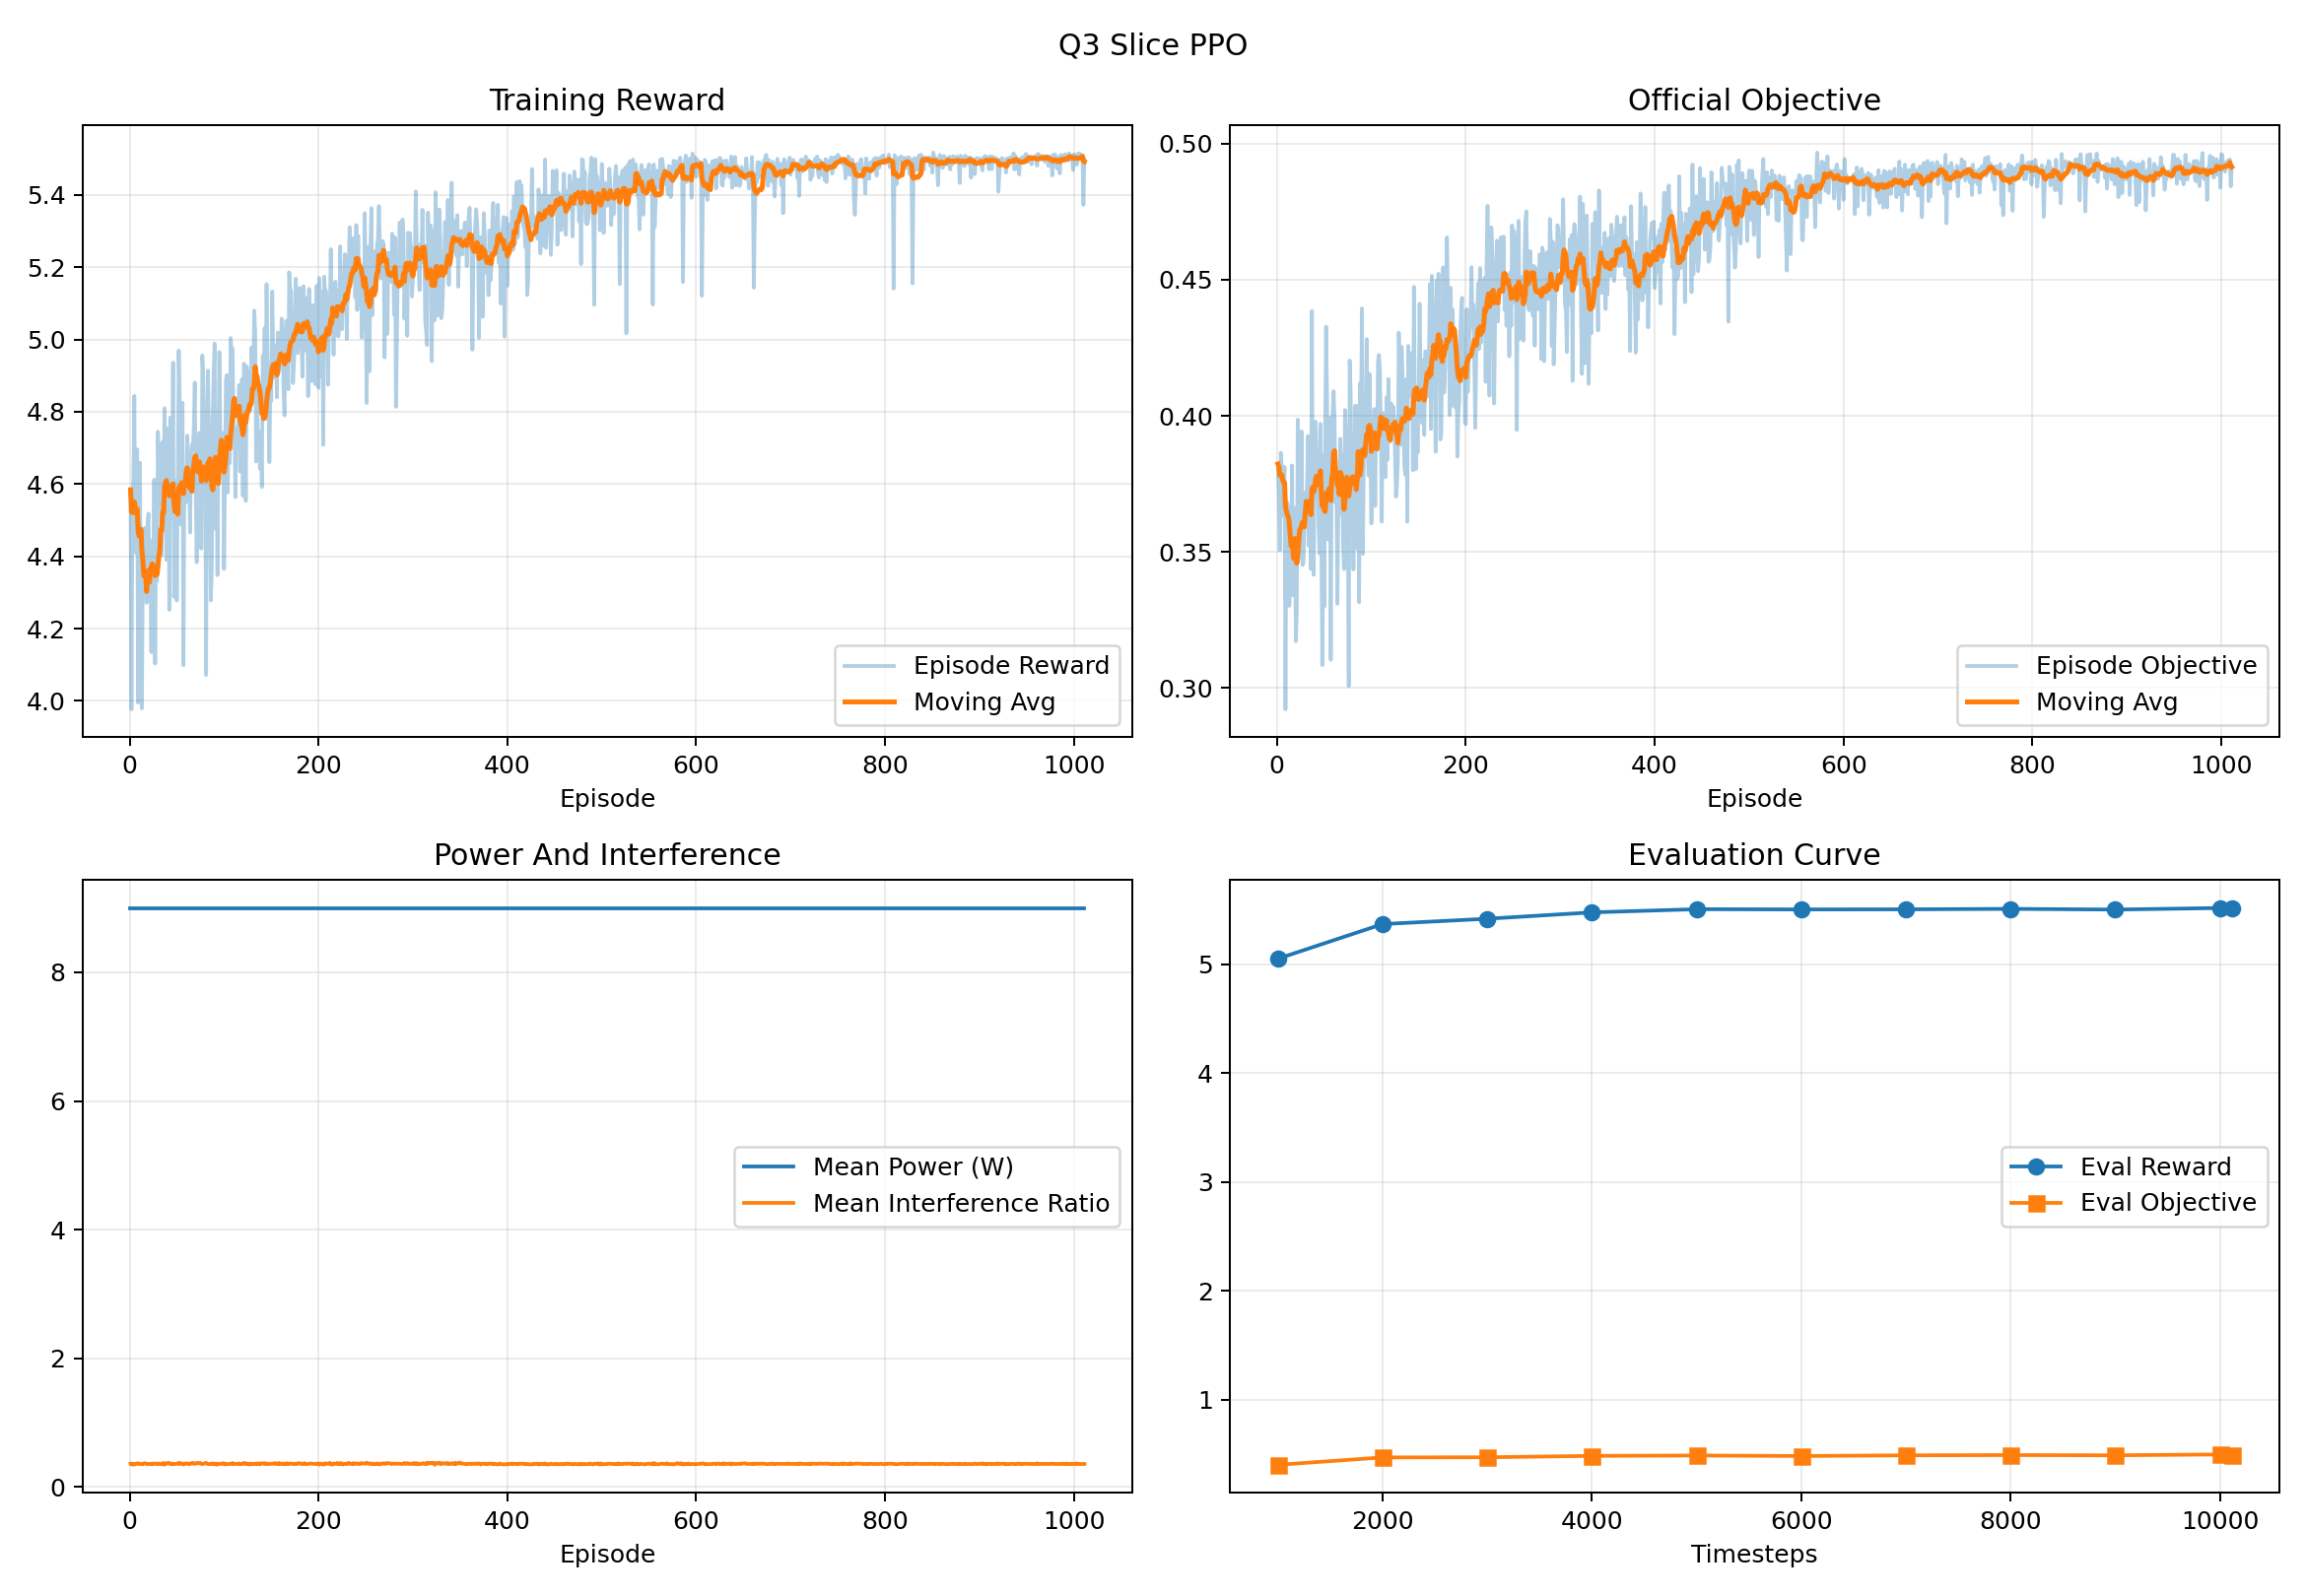
\includegraphics[width=0.95\linewidth]{q3_slice_seed17_convergence.png}
  \caption{seed=17切片层PPO训练曲线，评价目标值随训练推进整体上升。}
  \label{fig:q3_slice_convergence}
\end{figure}

\subsection{参数灵敏度分析}

效用函数中的$\alpha_u$与$\beta=(\beta_u,\beta_e,\beta_m)$为仿真场景校准常数，本文对其进行了参数扰动分析。动态单站在\texttt{channel\_data等2个文件(1)/channel\_data.xlsx}上以$lookahead=2$运行；多站在各组参数下重新训练切片层和功率层PPO（固定$seed=17$、训练步数$10000$、评估回合数1）。

\begin{table}[htbp]
  \centering
  \small
  \caption{动态单站滚动优化的参数灵敏度}
  \label{tab:q2_sensitivity}
  \resizebox{\linewidth}{!}{%
  \begin{tabular}{ccccc}
    \toprule
    扰动类型 & 参数取值 & 目标值 & 丢弃数(URLLC/eMBB/mMTC) & eMBB平均速率(Mbps) \\
    \midrule
    $\alpha_u$ & 0.90 & 0.8328 & 1/121/149 & 51.33 \\
    $\alpha_u$ & 0.93 & 0.8831 & 1/46/0 & 45.02 \\
    $\alpha_u$ & 0.95 & 0.8986 & 1/25/0 & 45.00 \\
    $\alpha_u$ & 0.97 & 0.9134 & 1/25/0 & 45.09 \\
    \midrule
    $\beta$ & (4,2,1) & 0.9044 & 1/25/0 & 45.00 \\
    $\beta$ & (5,3,1) & 0.8986 & 1/25/0 & 45.00 \\
    $\beta$ & (6,4,2) & 0.8928 & 1/25/0 & 45.00 \\
    \bottomrule
  \end{tabular}}
\end{table}

表\ref{tab:q2_sensitivity}显示，动态单站对$\alpha_u$更敏感：$\alpha_u$从$0.90$升至$0.97$，目标值从$0.8328$升至$0.9134$，eMBB和mMTC丢弃数明显下降。原因不仅仅是评价尺度改变——滚动优化在不同URLLC时延折扣下会重新选择切片预算，从而改变后续队列状态。在$\beta$扰动下，三组实验的完成数和丢弃数完全一致，目标值仅随惩罚强度重新标定而单调变化，说明在考察的$\beta$范围内策略输出较为稳定。

\begin{table}[htbp]
  \centering
  \small
  \caption{多站分层PPO的参数灵敏度}
  \label{tab:q3_sensitivity}
  \resizebox{\linewidth}{!}{%
  \begin{tabular}{cccccc}
    \toprule
    扰动类型 & 参数取值 & 目标值 & 丢弃数(URLLC/eMBB/mMTC) & 平均功率(W) & 平均干扰比 \\
    \midrule
    $\alpha_u$ & 0.90 & 0.4802 & 0/587/10556 & 0.1032 & 0.3555 \\
    $\alpha_u$ & 0.93 & 0.4916 & 0/587/10556 & 0.1032 & 0.3555 \\
    $\alpha_u$ & 0.95 & 0.4995 & 0/587/10556 & 0.1032 & 0.3555 \\
    $\alpha_u$ & 0.97 & 0.5076 & 0/587/10556 & 0.1032 & 0.3555 \\
    \midrule
    $\beta$ & (4,2,1) & 0.5321 & 0/587/10556 & 0.1032 & 0.3555 \\
    $\beta$ & (5,3,1) & 0.4995 & 0/587/10556 & 0.1032 & 0.3555 \\
    $\beta$ & (6,4,2) & 0.2962 & 0/587/10556 & 0.0981 & 0.3616 \\
    \bottomrule
  \end{tabular}}
\end{table}

\begin{figure}[htbp]
  \centering
  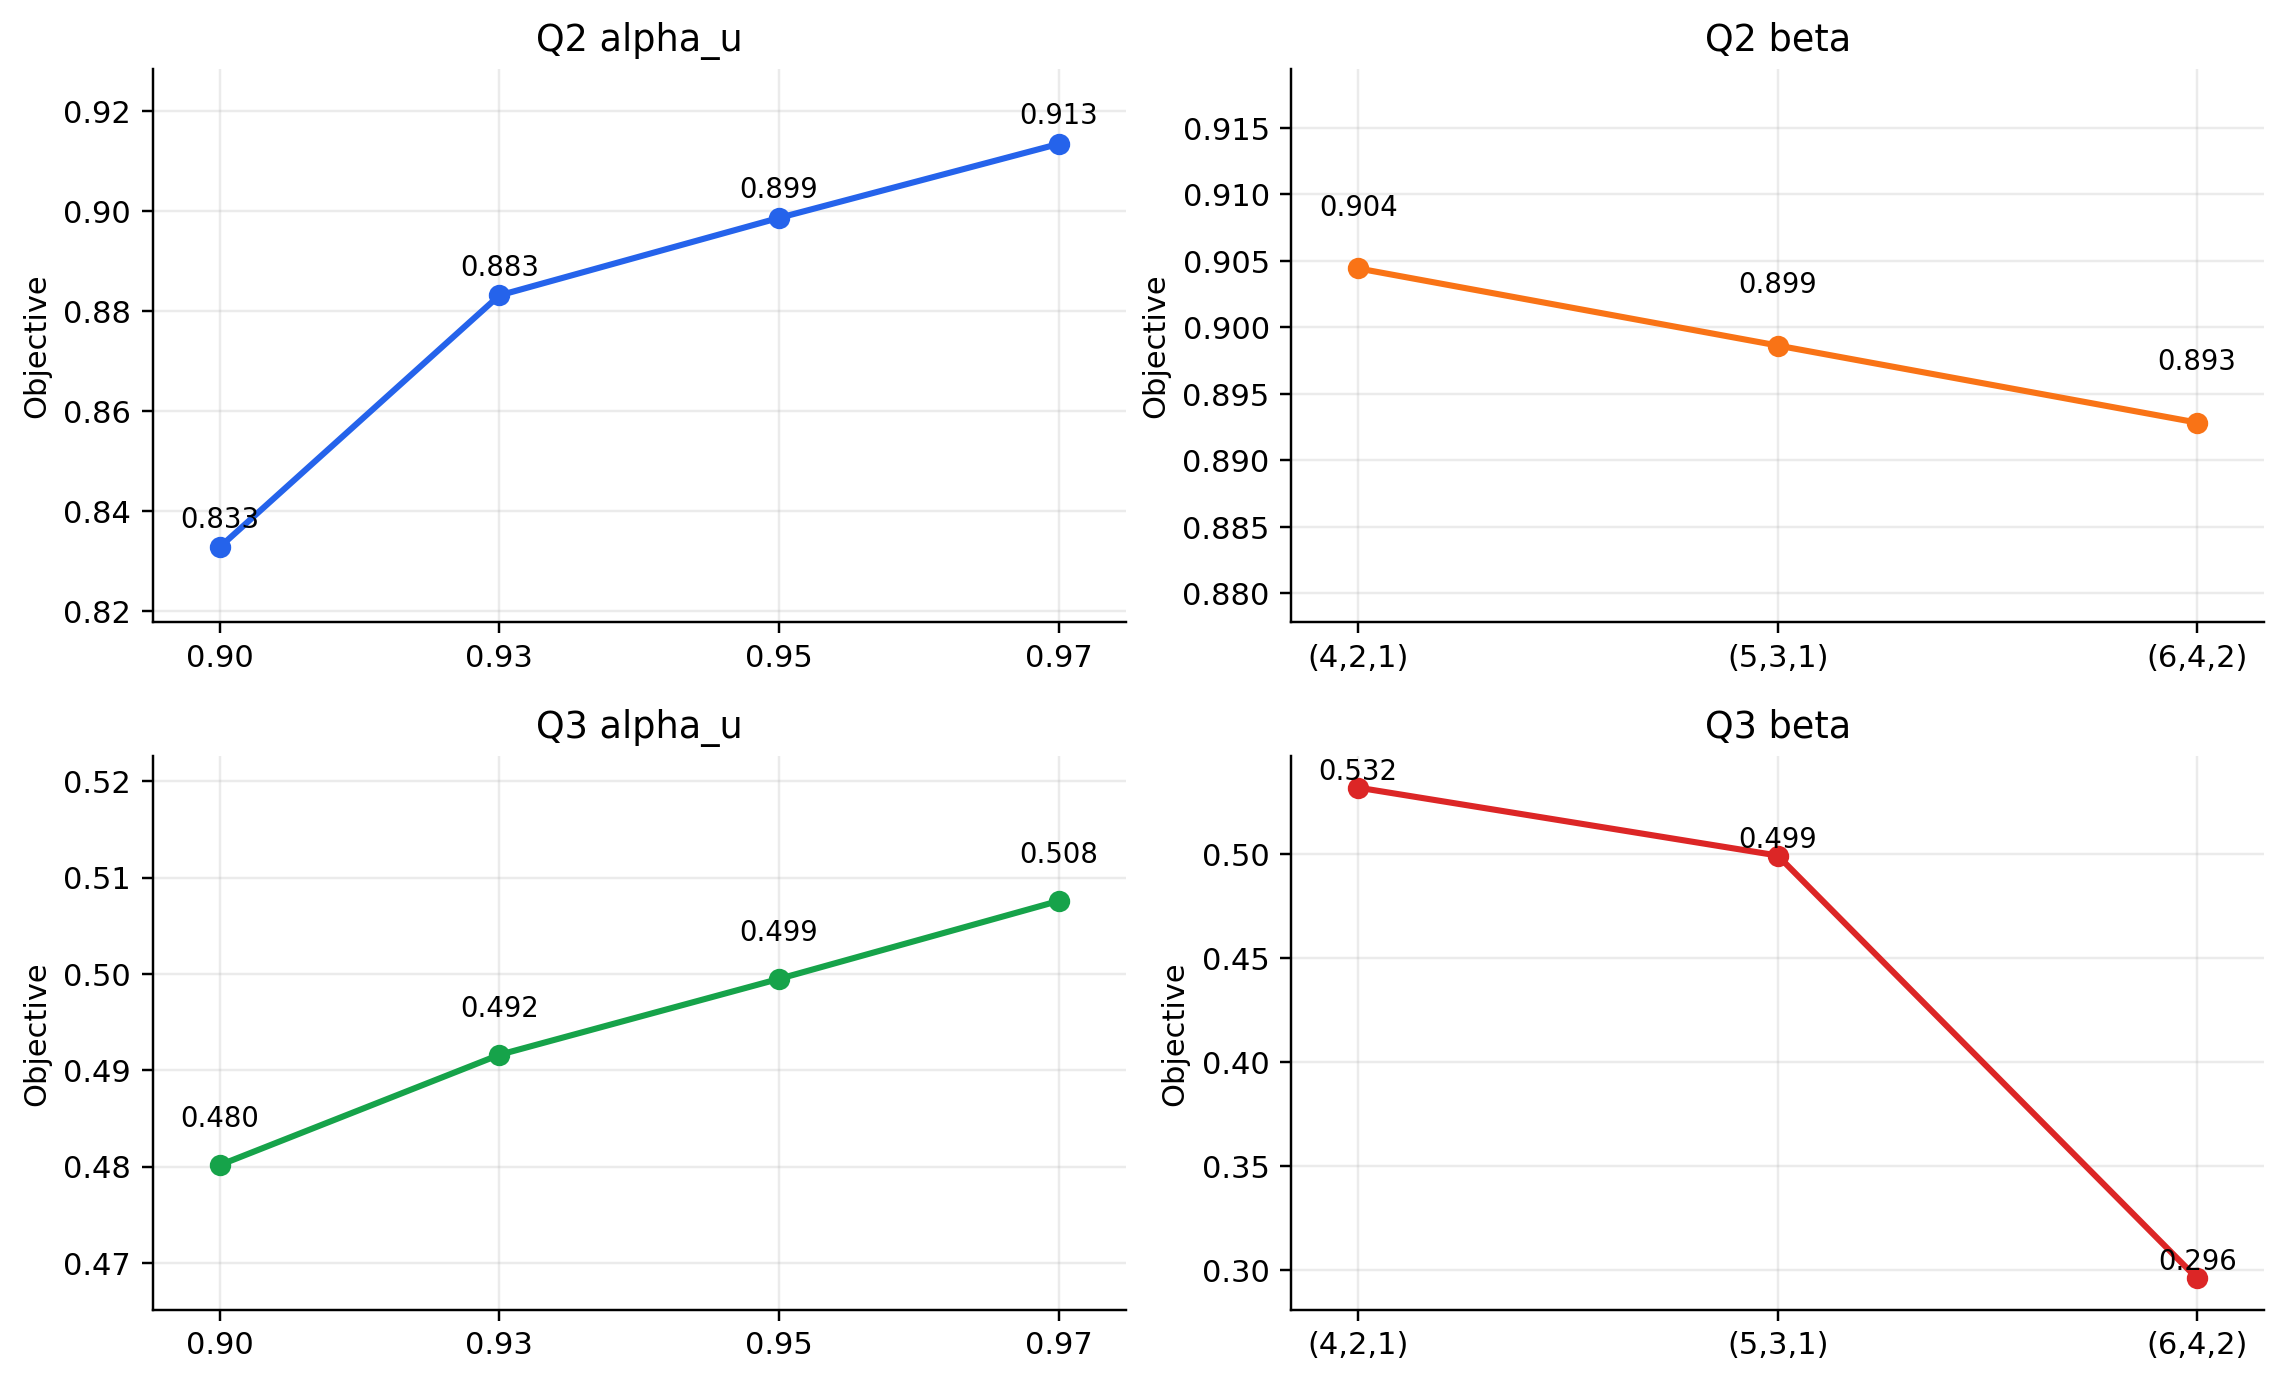
\includegraphics[width=0.95\linewidth]{sensitivity_objectives.png}
  \caption{动态单站与多站场景中$\alpha_u$和$\beta$扰动对综合目标值的影响。}
  \label{fig:sensitivity_objectives}
\end{figure}

表\ref{tab:q3_sensitivity}给出了多站场景验证。在$\alpha_u$扰动下，完成数、丢弃数、平均功率和干扰比均保持不变，目标值变化主要反映URLLC时延折扣的重新标定，策略行为未发生实质性变化。$\beta$扰动下，$(6,4,2)$使目标值降至$0.2962$，原因是eMBB和mMTC的大量丢弃被更高的惩罚系数放大。两个结论：(1) 在已考察参数范围内，URLLC零丢弃现象保持稳定；(2) mMTC服务不足并非单一默认参数造成，而是当前分层PPO策略和训练强度下的结构性短板。

\section{讨论}

\subsection{主要发现解读}

本文的三层递进式实验组织方式使得若干结论可以在对照中获得解读。

\textbf{时间前瞻的价值与边界。} Q2结果表明，将前瞻深度从1扩大到2窗口可以提升系统目标值，但从2到3却出现收益递减甚至略微恶化。这一现象的可能解释是：在$1000\,\mathrm{ms}$的有限时域和当前数据分布下，2步（$200\,\mathrm{ms}$）的前瞻已足以覆盖大部分URLLC和eMBB任务的完整生命周期，更深的预测增加了枚举搜索代价，也可能引入超出有效决策范围的信息扰动。

\textbf{分层分解的有效性与功率层的局限。} Q3主结果表明，分层PPO相对均匀分配和轻量级层次AC基线更稳定；但切片层单独评估（$0.4975$）与完整分层方法（$0.4995$）的差距仅约$0.002$，说明功率控制层在当前设置下不是主要QoS增益来源。更准确的解释是：功率层将平均发射功率从$9.0000\,\mathrm{W}$降至$0.1032\,\mathrm{W}$，同时基本保持服务目标不变。这并不意味着功率控制不重要，而是说明当前场景需要更丰富的干扰模式（如更密集的基站布局、更激进的频率复用策略）才能更充分地展示功率协调的服务质量收益。

\textbf{mMTC服务不足的根因。} mMTC完成率约$50\%$，而URLLC为零丢弃。从资源配置角度看，mMTC的每任务仅占用2个RB——看起来最"便宜"——但$500\,\mathrm{ms}$的宽松时延约束意味着队列可以不断积压。在有限时域$1000\,\mathrm{ms}$的终端惩罚压力下，策略更倾向于尽早完成URLLC和eMBB（时延约束紧、惩罚重），mMTC任务被不断推迟直至超时。灵敏度分析显示，在已考察的$\alpha_u$和$\beta$扰动范围内，mMTC服务不足现象没有被根本改变，说明它更接近当前策略结构和训练强度下的结构性结果，而非单一参数选择所致。

\subsection{局限性}

本文工作存在以下局限：(1) 接入模式采用最近基站规则，实际接入基站选择应纳入优化，尤其是在用户处于小区边缘、多基站信号质量接近的情况下；(2) 功率控制层在当前数据中主要体现为降功率而非提升服务目标，该层的QoS增益尚未被充分释放；(3) Q3每个模型仅使用一次确定性评估回合，在$1000\,\mathrm{ms}$时域内的随机波动可能掩盖部分方法差异；(4) 仿真数据为预设场景而非真实测量，结论向实际部署的迁移需要进一步验证；(5) mMTC完成率的提升尚未找到有效的算法路径，是本文遗留的最主要未解决问题。

\section{结论}

本文面向5G微基站无线接入侧，研究了双时间尺度切片预算与功率控制的协同优化问题。主要完成以下工作：

\begin{enumerate}[leftmargin=2em]
  \item 构建了同时纳入异构切片SLA、固定RB颗粒度、双时间尺度任务演化和跨站干扰耦合的统一优化模型。
  \item 设计了从静态枚举校准、动态滚动优化基线到分层PPO求解器的递进式方法链。
  \item 在预设仿真场景上验证了框架有效性：分层PPO多随机种子评估均值$0.4960\pm0.0031$，稳定优于均匀分配基线（$0.4740$）和线性AC基线（$0.4553$），且实现URLLC零丢弃。
  \item 通过消融实验和参数灵敏度分析，诚实报告了功率层主要带来低功率可行性、服务目标增益有限（$\sim0.002$）和mMTC服务不足（完成率约$50\%$）的当前边界。
\end{enumerate}

未来工作可沿以下方向展开：将接入基站选择纳入优化变量；在更密集的基站布局或更激进的频率复用策略下重新评估功率控制层的价值；引入多智能体协同机制以改善三类切片间的资源公平性；以及尝试将训练时域扩展到$1000\,\mathrm{ms}$以上，缓解终端惩罚对mMTC造成的系统性偏向。

\bibliographystyle{unsrt}
\bibliography{references}

\end{document}
